\section{Recap: Latent variable models}

\begin{frame} 
\mode<presentation>{
    \begin{center} \huge
        \secname
    \end{center}
}
    \begin{center}
    Latent variable models: an abstraction of Gaussian Mixture Models
    \end{center}
	
\end{frame}

%%%%%%%%%%%%%%%%%%%%%%%%%%%%%%%%%%%%%%%%%%%%%%%%%%%%%%%%%%%%%%%

\begin{frame}{}

\begin{center}
	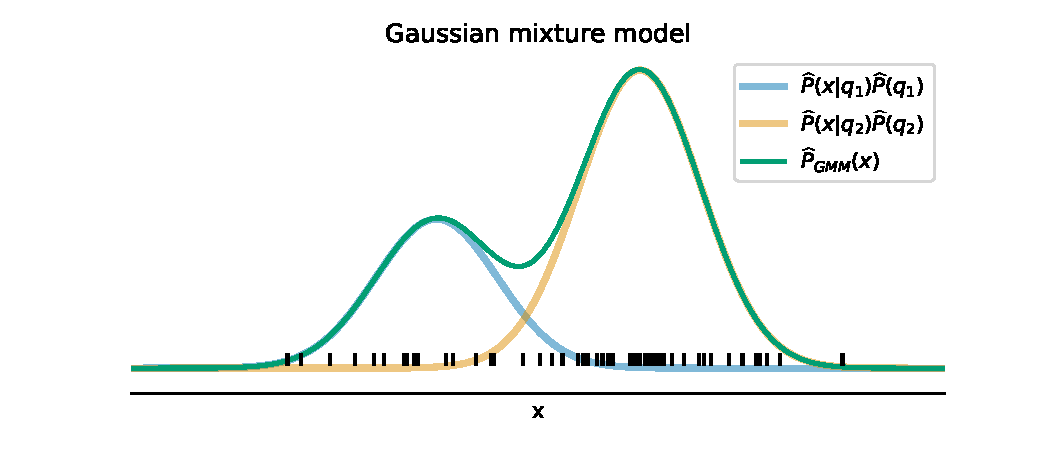
\includegraphics[width=0.7\textwidth]{img/latentexample_gmm}
	\notesonly{\captionof{figure}{A Gaussian Mixture Model as a latent variable model}}
\end{center}

``Groups'' may exist in the data. There are \emph{hidden causes} in the observations. We need a fit that accounts for this.

\end{frame}

\begin{frame}{Assignment variables as latent variables}

A simple way to understand what latent variables represent is to view them as assignment variables to components that we need to estimate.

Example:\\

\begin{itemize} 
\item assignment variables: $\vec{m}^{(\alpha)} =  \big( m_1^{(\alpha)}, \dots, m_M^{(\alpha)} \big)^\top \in \left\{ 0, 1 \right\}^M$ \\
		\begin{align}
		m_q^{(\alpha)} &= 
		\begin{cases}
		1, & \text{if component } q \text{ has generated point}~\alpha\\
		0, & \text{otherwise}
		\end{cases}
		%\hspace{0.5cm}
		\;\text{with} \;
		 \sum_{q=1}^{M} m_q^{(\alpha)} = 1 
		\end{align}
\end{itemize}

\end{frame}

\begin{frame}{Gaussian Mixture Models are latent variable models}

\slidesonly{
\begingroup
\small
\begin{itemize} 
\item assignment variables: $\vec{m}^{(\alpha)} =  \big( m_1^{(\alpha)}, \dots, m_M^{(\alpha)} \big)^\top \in \left\{ 0, 1 \right\}^M$ \\
		\begin{align}
		m_q^{(\alpha)} &= 
		\begin{cases}
		1, & \text{if component } q \text{ has generated point}~\alpha\\
		0, & \text{otherwise}
		\end{cases}
		%\hspace{0.5cm}
		\;\text{with} \;
		 \sum_{q=1}^{M} m_q^{(\alpha)} = 1 
		\end{align}
\end{itemize}
\endgroup
}

\notesonly{We have also seen how Gaussian Mixture Models can model assignment variables using mixture components.}

\begin{center}
	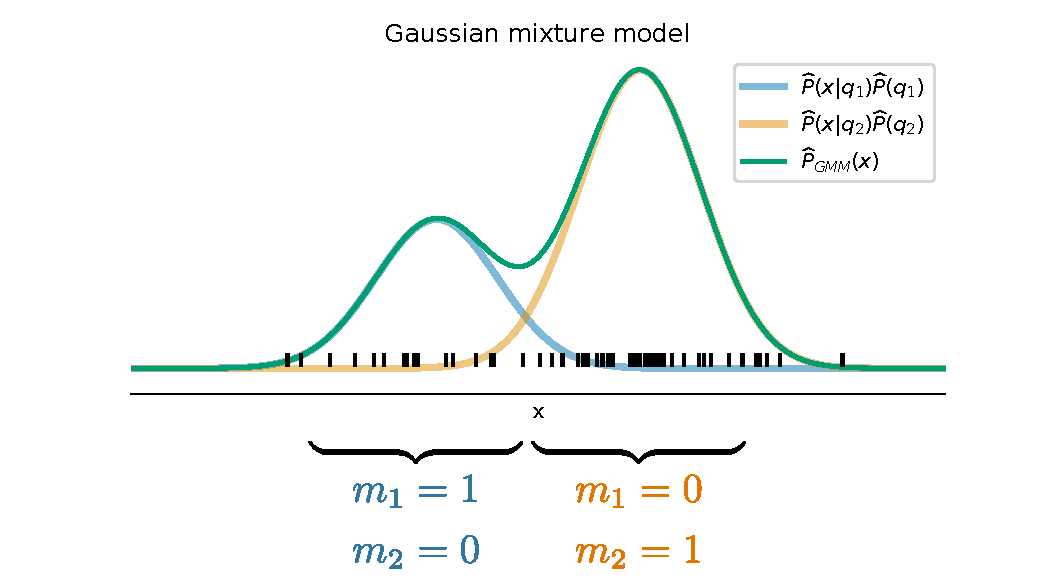
\includegraphics[width=0.7\textwidth]{img/latentexample_gmm_annot}
	\notesonly{\captionof{figure}{A Gaussian Mixture Model as a latent variable model with values of the assignment variables for the different groups in the data.}}
\end{center}


\end{frame}
